\documentclass[12pt, oneside]{article}
\usepackage[letterpaper, margin=1in, headsep=0.5in]{geometry}
\usepackage[english]{babel}
\usepackage[utf8]{inputenc}
\usepackage{amsmath}
\usepackage{amsfonts}
\usepackage{amssymb}
\usepackage{tikz}
\usetikzlibrary{quotes, angles}
\usepackage{graphicx}
%\usepackage{pgfplots}
%\pgfplotsset{width=10cm,compat=1.9}
%\usepgfplotslibrary{statistics}
%\usepackage{pgfplotstable}
%\usepackage{tkz-fct}
%\usepackage{venndiagram}
\usepackage{multicol}

\usepackage{fancyhdr}
\pagestyle{fancy}
\fancyhf{}
\rhead{\thepage \\Name: \hspace{1.5in}.\\}
\lhead{BECA / Dr. Huson / 10th Grade Geometry\\* 26 November 2018}

\renewcommand{\headrulewidth}{0pt}

\begin{document}
\subsubsection*{Do Now: Trigonometric ratios}
Show each step, justify each by writing the name of a theorem to the right.  \begin{enumerate}

  \item Given right $\triangle ABC$ with $AC=6, BC=3, AB=6.71$, $m\angle C=90^\circ$. Express each trig ratio as a fraction, then as a decimal to the nearest thousandth.
    \begin{center}
      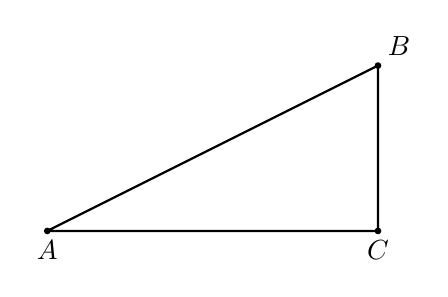
\begin{tikzpicture}[scale=0.7]
        \draw [thick](0,0)--(6,0)--(6,3)--(0,0);
        \draw [fill] (0,0) circle [radius=0.05] node[below]{$A$};
        \draw [fill] (6,0) circle [radius=0.05] node[below]{$C$};
        \draw [fill] (6,3) circle [radius=0.05] node[above right]{$B$};
        %\draw [color=blue] (0,0) ++(0.75,0) arc [start angle=0, end angle=70, radius=0.75];
        %\draw [color=blue] (4,0) ++(-0.22, 0.73) arc [start angle=110, end angle=180, radius=0.75];
        %\draw [thick] (0.8,3.1)--(1.2,2.9); %tick mark
        %\draw [thick] (2.8,2.9)--(3.2,3.1); %tick mark
        %\node [right] at (3.25,2.5){$x+7$};
        %\node [left] at (0.75,2.5){$2x+1$};
      \end{tikzpicture} \vspace{.1cm}
    \end{center}
    \begin{multicols}{2}
      \begin{enumerate}
        \item $\sin A = $ \vspace{1cm}
        \item $\cos A =$
        \item $\sin B = $ \vspace{1cm}
        \item $\tan B =$
      \end{enumerate}
    \end{multicols}

    \item Express the result to the nearest thousandth.  \vspace{.5cm}
      \begin{multicols}{2}
        \begin{enumerate}
          \item $\cos 60^\circ = $ \vspace{1cm}
          \item $\sin 67^\circ =$
          \item $\cos 23^\circ = $ \vspace{1cm}
          \item $\tan 45^\circ =$
        \end{enumerate}
      \end{multicols} \vspace{1cm}

\item Geometry 1st Trimester $+, \triangle$: What is working? What would you change?\\
Reflect on the first trimester. Write down one thing you think is working well for you. Write down one thing that you want to change.

\newpage
  \item Given right $\triangle JKL$ with $\overline{JK} \perp \overline{KL}$, $JL=7$, $m\angle J=20^\circ$.
    \begin{center}
      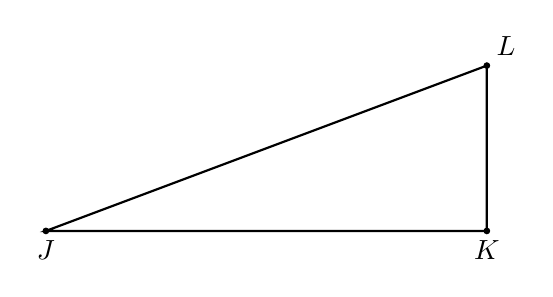
\begin{tikzpicture}[scale=0.7]
        \draw [thick](-1,0)--(7,0)--(7,3)--cycle;
        \draw [fill] (-1,0) circle [radius=0.05] node[below]{$J$};
        \draw [fill] (7,0) circle [radius=0.05] node[below]{$K$};
        \draw [fill] (7,3) circle [radius=0.05] node[above right]{$L$};
        %\draw [color=blue] (0,0) ++(0.75,0) arc [start angle=0, end angle=70, radius=0.75];
        %\draw [color=blue] (4,0) ++(-0.22, 0.73) arc [start angle=110, end angle=180, radius=0.75];
        %\draw [thick] (0.8,3.1)--(1.2,2.9); %tick mark
        %\draw [thick] (2.8,2.9)--(3.2,3.1); %tick mark
        %\node [right] at (3.25,2.5){$x+7$};
        %\node [left] at (0.75,2.5){$2x+1$};
      \end{tikzpicture} \vspace{1cm}
    \end{center}
    \begin{enumerate}
      \item Find the length $JK$\\[3cm]
      \item Find the length $KL$\\[2cm]
    \end{enumerate}

    \item Spicy: Given a rectangle with area 35, width $x$, and length $x+2$.
      \begin{enumerate}
        \item Find $x$.\\[4cm]
        \item Find the perimeter of the rectangle.
      \end{enumerate}

\end{enumerate}
\end{document}
